\subsection{Systemanalyse und -entwurf}

Aufbauend auf die Anforderung, einen Prototypen mit den Technologien der SAP Leonardo IoT Foundation zu entwickeln, wird in diesem Kapitel die zugrundeliegende Systemarchitektur untersucht. Dabei erfüllt die Analyse mehrere Zwecke. Zum einen wird die Forschungsfrage FF-1.2 (s. \ref{problemstellung}), welche Möglichkeiten zur intelligenten Vernetzung die Architektur bietet, beantwortet. An die Beantwortung dieser Frage knüpft sich die Prüfung der Kompatibilität der Zielarchitektur mit der \ac{rami}. In der Anforderungsanalyse wurde hauptsächlich die Anwendung des cloud-basierten Ansatzes als Lösung (s. \ref{technischeraufbau}) spezifiziert. Aus diesem Grund wird auf Grundlage der Analyse die angepasste Architektur des Zielsystems als Lösung für den technischen Aufbau entworfen.

\subsubsection{Systemarchitektur}

Wie in Abschnitt \ref{leo} beschrieben, bietet die SAP Leonardo IoT Foundation zahlreiche Dienste zur Integration von physischen Geräten in die SAP Cloud Platform und somit in die Geschäftswelt. Somit entstehen \ac{cpss}, welche im Rahmen eines \ac{iot}-Projektes typischerweise drei Phasen durchlaufen: \textit{Datentransport, Datenhaltung und Analyse} (s. Abschnitt \ref{technologien}). Wie die Architektur der SAP Leonardo IoT Foundation diesen Integrationsprozess bewerkstelligt, ist in Abbildung \ref{saparch} zu sehen. Die realen Geräte senden ihre Daten über \textit{Gateways} mit verschiedenen Netzwerkprotokollen an die \textit{SAP Cloud Platform Internet of Things Services} (1). Dort werden sie in einer PostgreSQL Datenbank gehalten \citep{Acharya2019}. Der Zugriff auf die Daten der \ac{cpss} erfolgt im Rahmen einer service-orientierten Architektur (SOA) über verschiedene \ac{api}. Um die Geräte in eine IoT-Anwendung zu integrieren, werden sie via \textit{Message Processing} an das \textit{IoT Application Enablement}\footnote{heute: \textit{SAP Leonardo IoT}} gesendet (2). Dort können digitale Zwillinge erstellt, funktionalisiert und analysiert werden. Für die Anwendungsentwicklung werden die Daten per OData- oder REST-Schnittstellen von der Cloud Foundry Umgebung an die WebIDE in der Neo Umgebung übergeben (3). Anschließend wird die Anwendung in die Cloud Foundry deployed. Die einzelnen Komponenten und Konzepte werden im Folgenden näher im Detail erläutert.

\begin{figure}[ht!]
  \centering
 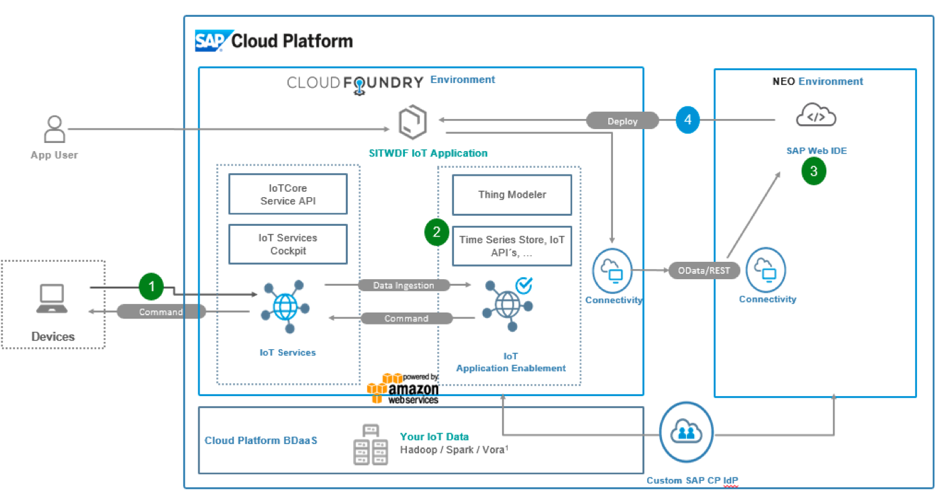
\includegraphics[width=1.05 \linewidth]{sap_architecture.png}
  \caption[Architektur von SAP]{Architektur von SAP \citep{Ganz2019}}
  \label{saparch}
\end{figure}

\newpage
\subsubsection{Datentransport: Internet of Things Gateway} \label{datentransport}

  Der erste Schritt von einem realen physischen Ding zu einem \ac{cpss} ist der Datentransport zu einem Datenobjekt im Netz (s. \ref{technologien}). Bezogen auf \ac{rami} und das Konzept der \acf{i40} ist dies der Prozess der Integration und Kommunikation. Das reale Objekt wird an ihre Verwaltungsschale angebunden, um virtuell repräsentiert werden zu können. Die Architektur von SAP bietet für diesen Vorgang zwei Möglichkeiten. Entweder den direkten Transport der Daten in die Cloud über die \textit{Gateway Cloud} oder über die \textit{Internet of Things Edge Platform}. Neben dem Senden von Messwerten in die Cloud können außerdem aus der Cloud heraus Befehle an das Gerät gesendet werden. Welche Variante auszuwählen ist, hängt von individuellen Anwendungsfällen und benötigten Protokollen ab. Die \textit{Gateway Cloud} wird in dem \textit{SCP Internet of Things Service} standardmäßig für MQTT und REST mitgeliefert.
  
  \begin{table}
    \centering
    \begin{tabular}{ccc}\\\toprule
    Protokoll & Cloud & Edge \\\midrule
    MQTT &x & x\\  \midrule
    HTTP (REST) & x & x\\  \midrule
    CoAP& & x\\  \midrule
    File &  & x\\  \midrule
    Modbus & & x\\  \midrule
    OPC UA & & x\\  \midrule
    SigFox & & x\\  \midrule
    SNMP & & x\\  \bottomrule
    \end{tabular}
    \label{protocol}
    \caption{Gateway-Protokolle}\label{gateway}
  \end{table}
 
  \noindent Die \textit{Internet of Things Edge Platform} wird von den Entwicklern lokal auf dem Gerät nach dem ausgewählten Kommunikationsprotokoll (s. Tabelle \ref{protocol}\footnote{Quelle: \citet{SAP2020}}) selbst konfiguriert. Sie dient dazu, Messwerte von Geräten mit mangelnder Internetverbindung zu verarbeiten und bei verfügbarerer Verbindung an die Cloud zu senden. In beiden Fällen werden die Nachrichten mit den Messwerten im \ac{json}- oder im \ac{protobuf}-Format mit POST-Anfragen an die API-Endpunkte der registrierten Geräte gesendet \citep{SAP2020}. Das Registrieren der Geräte wird im nächsten Kapitel näher behandelt. SAP bietet außerdem die Möglichkeit, das \textit{Internet of Things Service} mit dem \textit{Internet of Things Edge Platform SDK} zu erweitern. Das SDK bietet Tools auf Eclipse, das Gateway mit \textit{Interceptors} zu erweitern. Die Messwerte können vor dem Senden an die Cloud vom Gateway abgefangen, modifiziert oder gefiltert werden.
\newline
  \begin{lstlisting} [label=lst:endpunkt, caption=API-Endpunkte der Gateways]
    // Endpunkt der Gateway Cloud
    https://<HOST_NAME>:443/iot/gateway/rest/measures/<deviceAlternateId>
    // Endpunkt des Edge Gateways
    https://<IOT_GATEWAY_IP>:8699/measures/<deviceAlternateId>
  \end{lstlisting}

  %------------------------------------------


\subsubsection{Datenhaltung: SCP Internet of Things Service} \label{iotcp}

Wie in Listing \ref{lst:endpunkt} zu sehen ist, haben die Gateways, welche die Daten der Geräte an die Cloud übermitteln, eine \textit{deviceAlternateId} zum Ziel. Damit die Daten in der Cloud ankommen können, müssen die Geräte und Sensoren für die Messwerte im \textit{Internet of Things Service} der SAP Cloud Platform registriert werden. Für diesen Zweck liefert SAP ein Datenmodell für die Geräte, nach dem eine Entität des Geräts erstellt werden muss (s. Abbildung \ref{fig:devicemodel}). Nach dem Modell muss ein Gerät mindestens aus einem Sensor bestehen und eindeutig einem Gateway zugeordnet sein. Die Sensoren sind immer Instanzen von bestimmten Sensortypen, denen Fähigkeiten und Eigenschaften zugeordnet werden.
Für die Registrierung bietet das System zwei Möglichkeiten. Man es kann entweder über die grafische Benutzeroberfläche des \textit{IoT Services Cockpit} durch das Ausfüllen von Formularen erstellen oder über die \textit{IoT Core Service API} (s. Abbildung \ref{saparch}). In beiden Fällen werden POST-Anfragen im \ac{json}-Format an den API-Endpunkt des Tenants im \textit{Internet of Things Service} gesendet. Für diesen Zweck stellt SAP eine Sammlung von \textit{Device Management API} zur Verfügung. Nachdem die Geräte registriert wurden, kann die SAP Cloud Platform das Datenobjekt des \ac{cpss} halten. Somit befindet sich das physische Ding in der Informationsschicht nach \ac{rami}.

\begin{figure}[h]
  \centering
  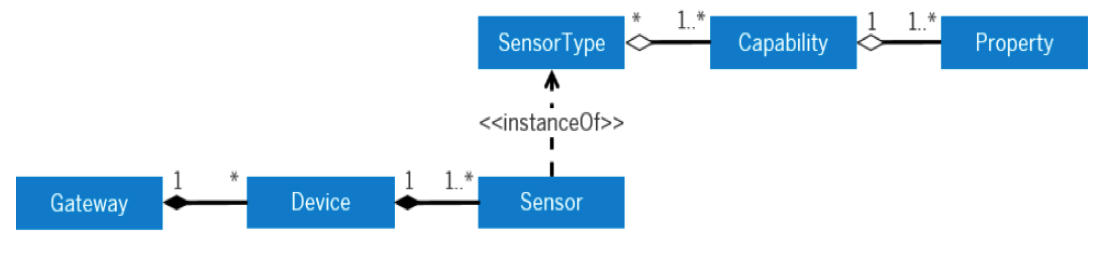
\includegraphics[width=1.0\linewidth]{pictures/device_model}
  \caption[Gerätemodell]{Gerätemodell}
  \label{fig:devicemodel}
\end{figure}

\noindent Genau so wie das Erstellen von Geräten über APIs, kann auf Messwerte und Eigenschaften der Geräte über GET-Anfragen an die API-Endpunkte zugegriffen werden. Der Zugriff auf die Daten nennt sich in diesem  Kontext \textit{Message Processing} und kann über die von SAP zur Verfügung gestellte Sammlung von \textit{Message Processing API} konfiguriert und abgerufen werden. Diese Schnittstellen sind vor allem hinsichtlich der Einbindung der Daten in externe Dienste und Anwendungen von großer Relevanz. Je nach Bedarf und Anwendungsfall können unterschiedliche Dienste konfiguriert werden \citep{SAP2020}:
\begin{itemize}
  \item \textit{SAP Leonardo IoT Integration} für den Datentransfer an SAP Leonardo IoT
  \item \textit{SQL} für den Fall, dass die Gerätedaten in einer externen DB gespeichert werden sollen
  \item \textit{Kafka} z.B. für Big-Data Dienste
  \item \textit{HTTP}, um einen eigenen API-Endpunkt zu nutzen
\end{itemize}

\subsubsection{Analyse: SAP Leonardo IoT}

Über den Message Processing Service \textit{SAP Leonardo IoT Integration} werden die Daten der Geräte an SAP Leonardo IoT übergeben. Laut SAP bietet Leonardo IoT \glqq alle notwendigen Funktionen zum Einrichten von Thing- und Geschäftspartnerstrukturen als Repräsentation der realen Welt\grqq{} \citep[S. 11]{SAP2019}. Mit allen notwendigen Funktionen sind in diesem Fall eine Sammlung von REST- und OData-basierten Microservices gemeint, die zum Speichern und Bereitstellen der Daten dienen. In erster Linie dienen sie dazu, einen digitalen Zwilling mit dem \textit{Thing Modeler} des Geräts zu erstellen. Die folgende Abbildung (\ref{leoae}) gibt eine Übersicht über die Softwarearchitektur und die Interaktion mit verschiedenen Komponenten.
\begin{figure}[ht]
  \centering
  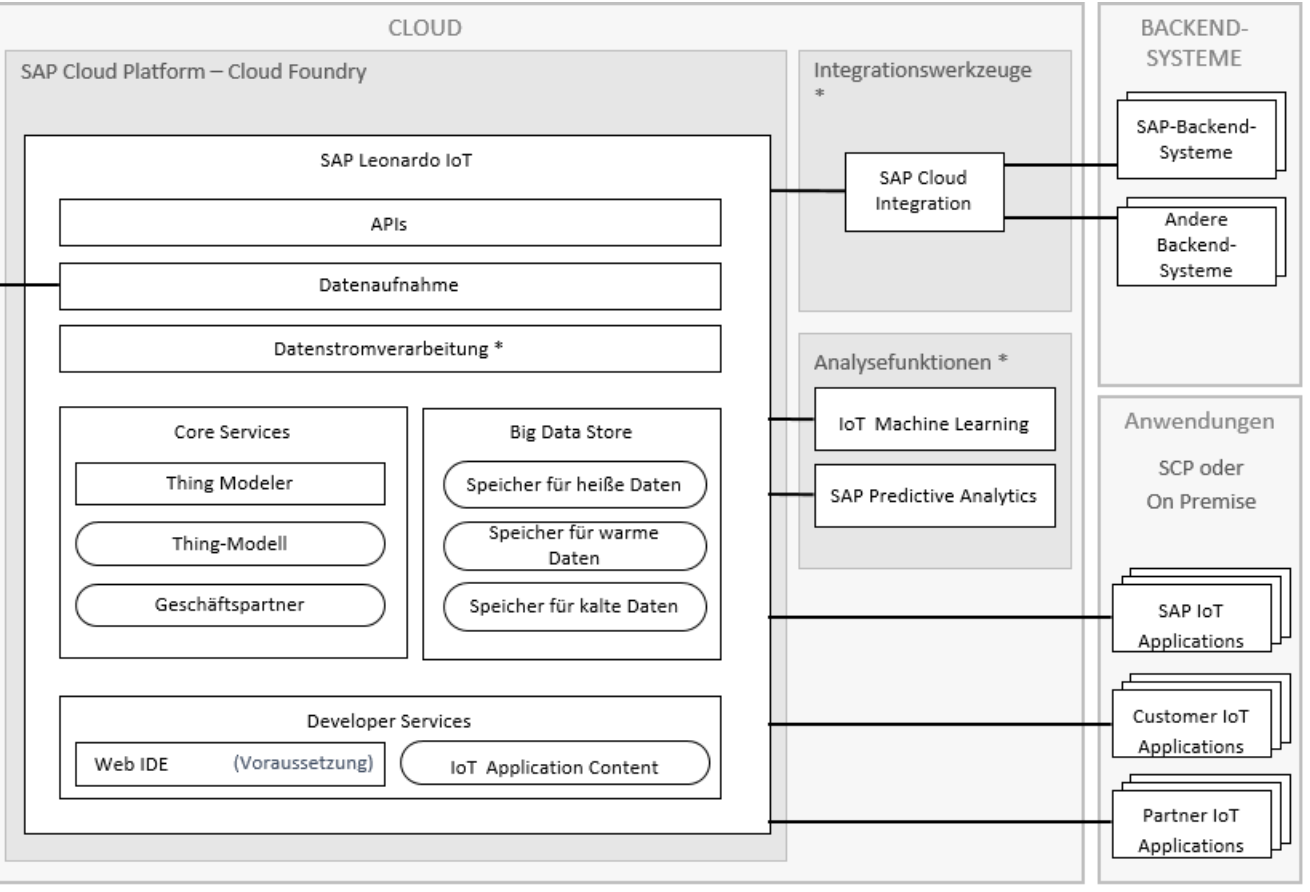
\includegraphics[width=1.0\linewidth]{pictures/leo_ae}
  \caption[Architekturübersicht SAP Leonardo IoT]{Architekturübersicht SAP Leonardo IoT \citep[S. 12]{SAP2019}}
  \label{leoae}
\end{figure}
 \noindent Mithilfe der API-Sammlung können zum Beispiel Geschäftspartner, Standorte, Berechtigungen oder Ereignisse zugeordnet werden. Dadurch wird dem \textit{Ding}, welches vorher rohe Daten erzeugt hat, eine Funktion und ein Zweck zugeordnet. Nach der \ac{rami} befände man sich somit in der Funktionsschicht. Eine weitere wichtige Funktion von SAP Leonardo IoT ist das \textit{Application Enablement}, welches die modellierten Zwillinge an die Web IDE der Neo Laufzeitumgebung sendet. Dort können mit Hilfe von Templates \textit{Freestyle IoT Applications} nach der UI5-Technologie von SAP erstellt werden. Außerdem dient SAP Leonardo IoT als Schnittstelle für weitere SaaS in unterschiedlichen Laufzeitumgebungen, für weitere Leonardo-Produkte mit Analysefunktionen oder für die Integration in Backend-Systeme. Allerdings handelt es sich bei SAP Leonardo um ein junges Projekt, welches die Funktionen zur Integration des Backend-Systems und die Einbindung der Analysefunktionen erst in Zukunft realisieren soll.

\subsubsection{Destinations}

Damit ein System mit Systemen aus verschiedenen Laufzeitumgebungen oder Endpunkten kommunizieren kann, werden in der SAP Cloud Platform Destinations erstellt. In der Abbildung \ref{saparch} kann man z.B. erkennen, dass zwischen der Cloud Foundry Umgebung und der Neo Umgebung eine Verbindung hergestellt wird (3), um Thing-Daten für die Anwendungsentwicklung zu transferieren. Damit die Neo Umgebung die Daten empfangen kann, muss dort eine HTTP-Destination erstellt werden. Diese muss aus einer Ziel-URL des Cloud Foundry Dienstes und kann aus Authentifizierungsmethoden sowie Anmeldeinformationen bestehen.

% Sicherheit
\subsubsection{Sicherheit}

Wie in Abschnitt \ref{general} beschrieben, trägt die Sicherheit in der Kommunikation in IoT-Netzwerken eine Schlüsselrolle. Insbesondere mit Blick auf die Architekturmodelle der Systemlandschaft (s. Abbildung \ref{saparch} und \ref{leoae}) wird deutlich, dass die Datenkommunikation im Rahmen einer \ac{soa} über zahlreiche Schnittstellen stattfindet. Der Zugriff auf diese Schnittstellen erfordert sichere Authentifizierungs- und Autorisierungsmaßnahmen. Die Infrastruktur von SAP stellt Standardmechanismen für die sichere Kommunikation zwischen den Komponenten zur Verfügung. Der Datentransport findet mit X509.1-Mechanismen asymmetrisch verschlüsselt über das \textit{\ac{tls}} Protokoll statt \citep{SAP2020a}. Um die Geräte im Internet of Things Service registrieren zu können, erhält jeder Tenant einen client-spezifischen \textit{private Key} im .pem- oder .p12-Format. Nur mit Angabe des Schlüssels können Edge Gateways so konfiguriert werden, dass über sie sicher mit dem Gerät kommuniziert werden kann. Auch der Zugriff auf die digitalen Zwillinge von SAP Leonardo IoT kann über das Berechtigungsmanagement eingeschränkt werden, sodass die Daten nach Verantwortlichkeiten getrennt werden. Der Zugriff auf die Ressourcen via API wird über die Autorisierung mit OAuth2.0 gesichert.

\subsubsection{Kompatibilität mit Referenzarchitektur}

Eine Anforderung an den Prototypen ist,  Kompatibilität mit der \ac{rami} und dem Konzept der Industrie-4.0-Komponente aufzuweisen. Im Zuge der Systemanalyse wurden bereits für einzelne Komponenten Referenzen zu einzelnen Schichten der IT-Sicht des \ac{rami} erstellt. Abbildung \ref{ramicustom} veranschaulicht die Referenzen zwischen den Schichten und den Komponenten des Systems.

\begin{figure}[H]
  \centering
  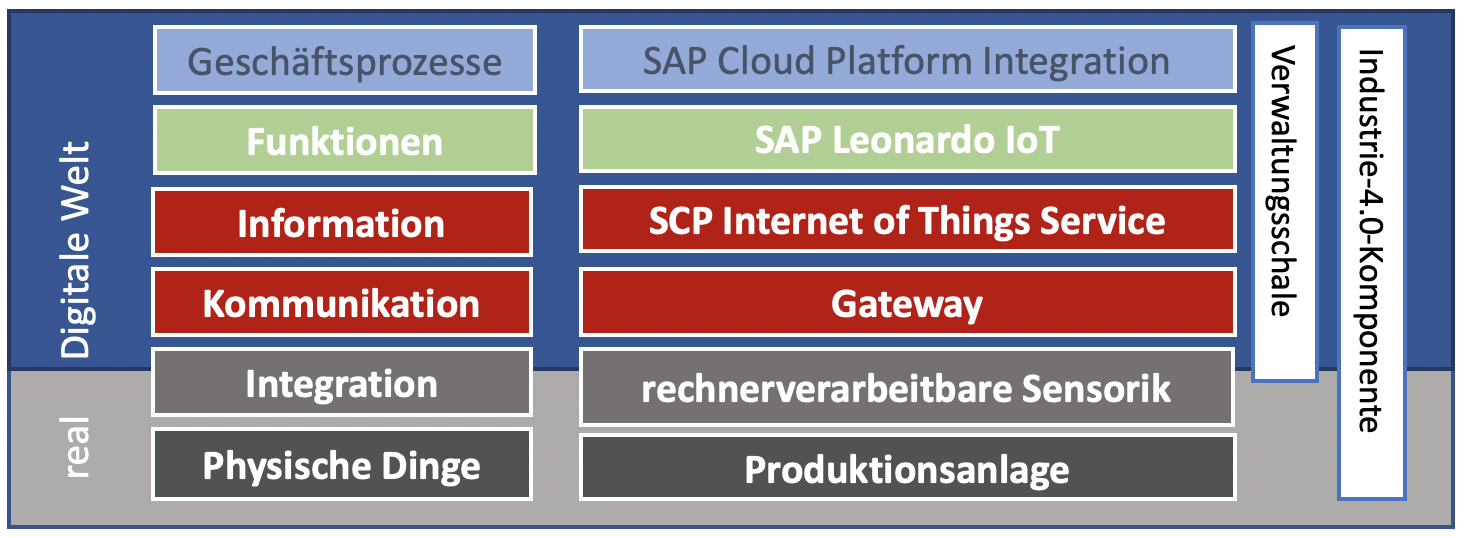
\includegraphics[width=1.0\linewidth]{pictures/ramicustom}
  \caption[Referenz zu den Schichten der RAMI 4.0]{Referenz zu den Schichten der RAMI 4.0}
  \label{ramicustom}
\end{figure}
 \noindent Die Produktionsanlage wird an ihre Verwaltungsschale über das Gateway angebunden. Somit kann das Objekt als Industrie-4.0-Komponente bezeichnet werden. Über den Dienst SAP Cloud Platform Integration kann die horizontale Integration der Industrie-4.0-Komponente in das Backend und somit in die Organisation und Geschäftsprozesse erfolgen.

\subsubsection{Systementwurf gemäß Architekturkonzept} \label{systementwurf}

Nach dem vorliegenden Architekturkonzept und den Anforderungen an das System ergibt sich die in Abbildung \ref{systemcustom} dargestellte Systemarchitektur. Sie spezifiziert sowohl die Komponenten des Systems als auch den Datenfluss. Für die Simulation einer Windenergieanlage wird ein Raspberry Pi über die IoT Edge Platform REST in die SAP Cloud Platform integriert. Die Daten des Geräts werden unter der deviceId der Entität in dem Internet of Things Service gehalten. Die grünen Pfeile visualisieren den Datenfluss von der Hardware über die SAP Cloud Plaform zu den Nutzern der IoT-Anwendung. Datenflüsse, die durch Anbindung von speziellen Microservices entstehen, werden durch die roten Pfeile repräsentiert. Dabei fließen die Daten durch die HTTP-Destinationen \textit{SMS\_Gateway, Led\_Blink\_Command und Standard\_EventType}. Ausgelöst werden die Funktionen der Destinationen von Regeln, die für bestimmte Messwerte definiert werden. Zum Beispiel kann der Eingang von kritischen Werten das Senden von Befehlen zum Aufleuchten der LED oder das Senden einer Benachrichtigungs-SMS auslösen. Im folgenden Kapitel wird die Umsetzung detailliert beschrieben.

\begin{figure}[H]
  \centering
  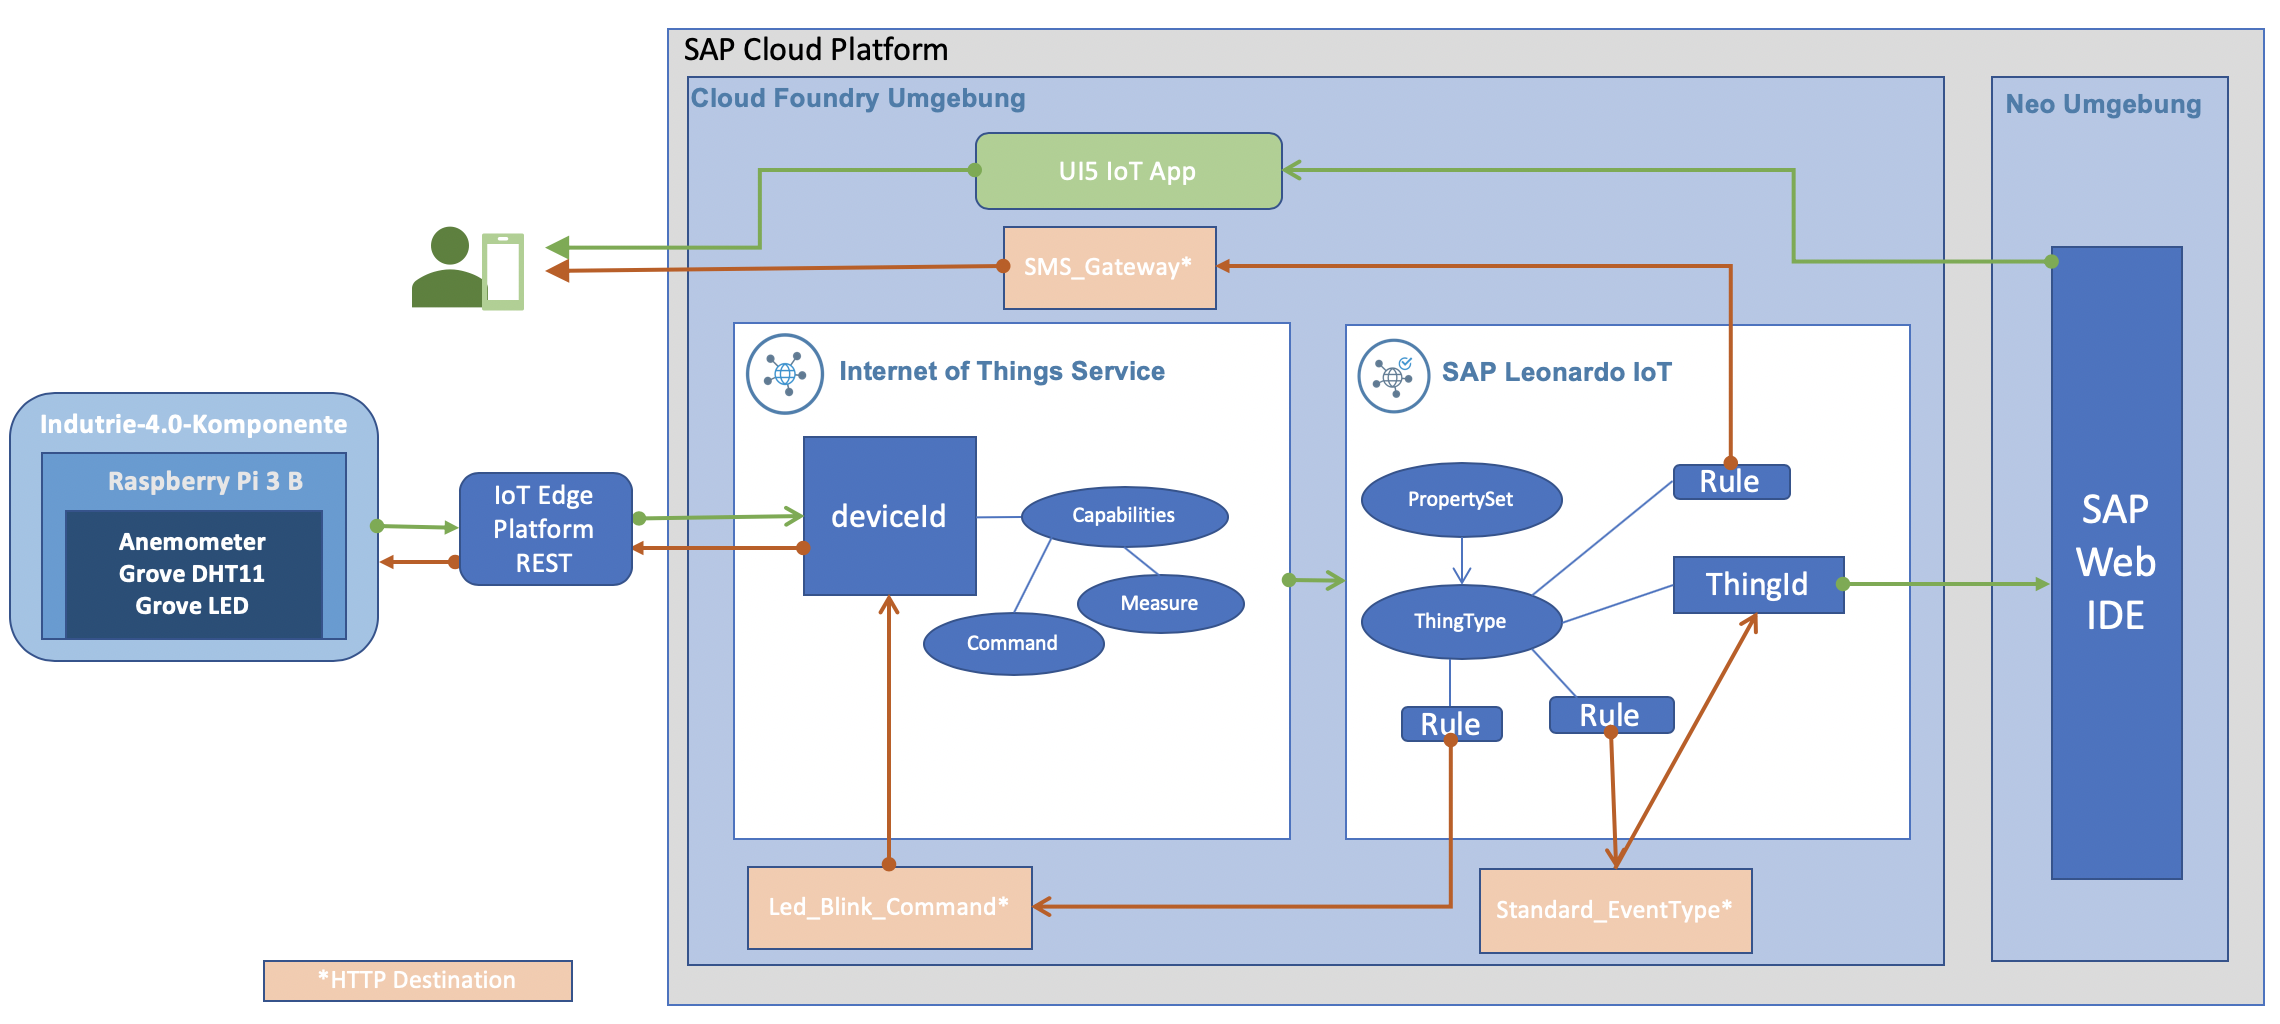
\includegraphics[angle=90, scale=0.5]{pictures/systemcustom}
  \caption[Systementwurf]{Systementwurf (eigene Darstellung)}
  \label{systemcustom}
\end{figure}


\newpage